% !TEX root = document.tex

\section*{Eidesstattliche Erklärung}
\addcontentsline{toc}{section}{Eidesstattliche Erklärung}

Wir erklären an Eides statt, dass wir unsere Hausarbeit \\ \\
\glqq \titel \grqq{} \\ \\
selbstständig und ohne fremde Hilfe angefertigt haben und dass wir alle von anderen Autoren wörtlich übernommenen Stellen wie auch die sich an die Gedankengänge anderer Autoren eng anlehnenden Ausführungen unserer Arbeit besonders gekennzeichnet und die Quellen zitiert haben.
\\ \\

\begin{figure}[!h]
	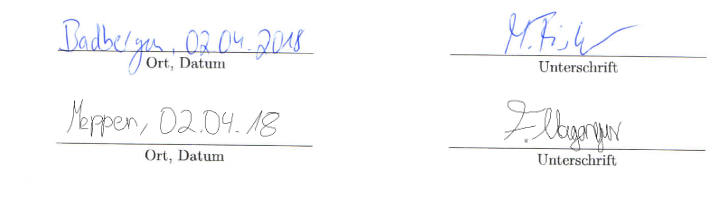
\includegraphics[width=\textwidth]{15.png}
\end{figure}